\apendice{Plan de Proyecto Software}

\section{Introducción}
En este apartado se incluye la explicación del desarrollo del proyecto a través de la planificación temporal mediante metodología ágil, el estudio de viabilidad y las viabilidades tanto económicas como legales del proyecto.

\section{Planificación temporal}
Para planificación temporal del desarrollo del proyecto se emplea la metodología ágil realizando sprints de una o dos semanas de duración, con el fin de realizar reuniones para el seguimiento del cumplimento de los objetivos establecidos en cada sprint, y la propuesta de las tareas a realizar en los siguientes sprints.

Para la gestión del proyecto se ha utilizado la herramienta Zube de GitHub lo que ha permitido la organización, la asignación y estimación de las tareas del proyecto de una forma sencilla y visual.

La estimación temporal de las tareas realizadas en cada sprint es asignada a partir de los story points de la siguiente forma:

\begin{table}[ht!]
    \centering
    \resizebox{8cm}{!} {
    \begin{tabular}{|c|c|}
    \hline
    \rowcolor[rgb]{0.99,0.93,0.93}
    \textbf{Story points}   & \textbf{Estimación temporal} \\ \hline
    \textbf{1}              & 30 minutos \\ \hline 
    \textbf{2}              &  2 horas \\ \hline
    \textbf{3}              &  5 horas \\ \hline 
    \textbf{5}              &  8 horas \\ \hline 
    \textbf{8}              & 12 horas \\ \hline 
    \textbf{13}              & 18 horas \\ \hline 
    \textbf{20}              & 22 horas \\ \hline 
   
    \end{tabular}}
    \caption{Estimación temporal de los story points.}
    \label{tab:my_label}
\end{table}
\newpage

\subsection{Sprint 1: 12/02/2023 - 25/02/2023}
La primera semana del sprint 1 fue empleada para la inicialización del proyecto, incluyendo la creación y configuración del repositorio, la familiarización e instalación de Zotero y la selección del editor de texto para la documentación. 

También se realizaron tareas de investigación para la búsqueda de trabajos relacionados y la selección de herramientas que se van a emplear para el desarrollo del proyecto.
Posteriormente, se realizó la creación de la máquina virutal, la instalación de PostgreSQL, Visual Studio Code, Python y Flask.

Por último, se documentaron las tareas realizadas en el sprint.

En este sprint se ha realizado un conjunto de tareas estimadas de 20 story points, y por tanto equivalente a 24 horas y 30 minutos.

\begin{table}[ht!]
    \centering
    \resizebox{15cm}{!} {
    \begin{tabular}{|l|c|c|}
    \hline
    \rowcolor[rgb]{0.99,0.93,0.93}
    \textbf{Tareas}     &\textbf{Tag}     & \textbf{Story points} \\ \hline
    \textbf{Creación y configuración del repositorio}         &\cellcolor[rgb]{0.93,0.35,0.0}\textcolor{white}{configuration}      &1 \\ \hline 
    \textbf{Familiarización e instalación de Zotero}         &\cellcolor[rgb]{0.6,1.0,0.6}research      &2 \\ \hline
    \textbf{Selección del editor de texto para documentación}         &\cellcolor[rgb]{0.6,1.0,0.6}research      &1 \\ \hline 
    \textbf{Búsqueda de trabajos relacionados}         &\cellcolor[rgb]{0.6,1.0,0.6}research      &3 \\ \hline 
    \textbf{Búsqueda y selección de herramientas}          &\cellcolor[rgb]{0.6,1.0,0.6}research      &3 \\ \hline 
    \textbf{Creación de máquina virtual}         &\cellcolor[rgb]{0.93,0.35,0.0}\textcolor{white}{configuration}      &2 \\ \hline 
    \textbf{Instalación PostgreSQL}         &\cellcolor[rgb]{0.93,0.75,0.0}\textcolor{white}{install}      &1 \\ \hline 
    \textbf{Instalación Visual Studio Code}         &\cellcolor[rgb]{0.93,0.75,0.0}\textcolor{white}{install}      &1 \\ \hline 
    \textbf{Instalación Python y Flask}         &\cellcolor[rgb]{0.93,0.75,0.0}\textcolor{white}{install}      &1 \\ \hline 
    \textbf{Documentación de las tareas realizadas en el sprint}         &\cellcolor[rgb]{0.0,0.33,0.71}\textcolor{white}{documentation}      &5 \\ \hline 
    \end{tabular}}
    \caption{Tareas completadas del Sprint 1.}
    \label{tab:my_label}
\end{table}
\newpage
\begin{figure}[htb]
    \centering
    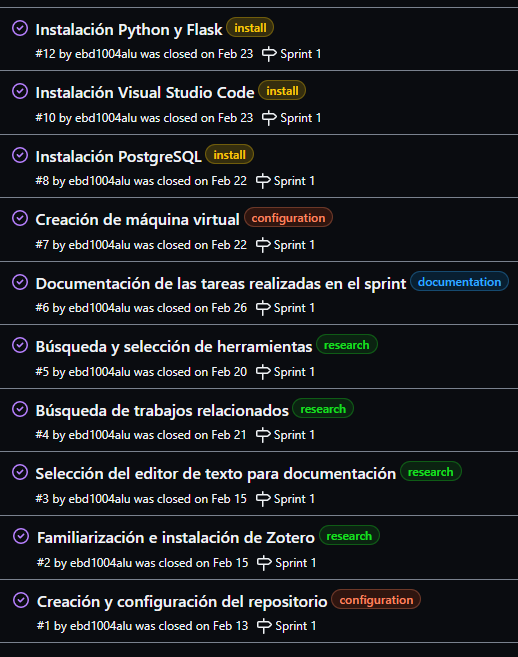
\includegraphics[width=0.9\textwidth]{Sprint1}
    \caption{Issues sprint 1.}
    \label{fig:Sprint1}
\end{figure}
\newpage

En el siguiente gráfico se podría ver el progreso del trabajo durante el sprint, pero debido a un problema que surgió con la herramienta de Zenhub se perdió el progreso de este sprint.
\begin{figure}[htb]
    \centering
    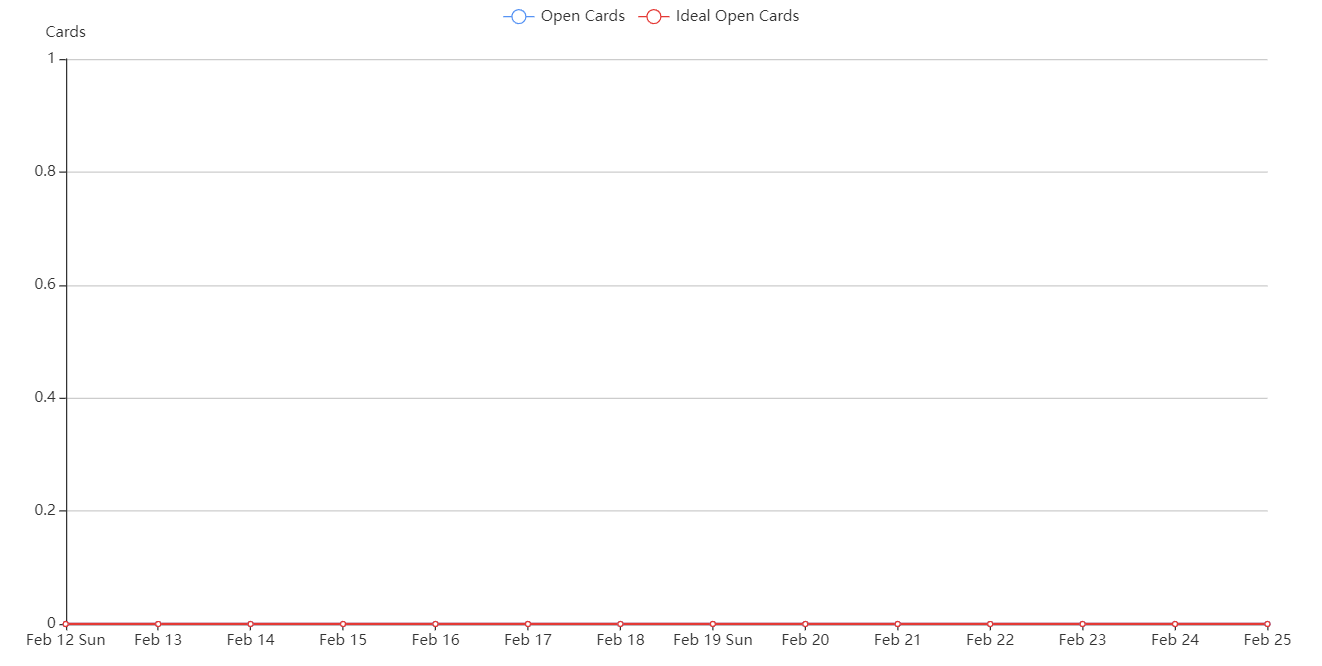
\includegraphics[width=1.1\textwidth]{burndown_1}
    \caption{Burndown del sprint 1.}
    \label{fig:burndown_1}
\end{figure}

\subsection{Sprint 2: 26/02/2023 - 11/03/2023}
La primera semana del sprint 2 fue empleada para el desarrollo del prototipo de la aplicación web.

Posteriormente, se empezó a realizar el desarrollo del registro e inicio de sesión y la creación de las distintas tablas que iba a contener la base de datos. Estas dos últimas tareas debido a diversos problemas no se pudieron terminar a tiempo en este sprint por lo que se continuaron en el siguiente sprint.

Por último, se documentaron las tareas realizadas en el sprint.

En este sprint se ha realizado un conjunto de tareas estimadas de 18 story points, y por tanto equivalente a 27 horas.

\begin{table}[ht!]
    \centering
    \resizebox{15cm}{!} {
    \begin{tabular}{|l|c|c|}
    \hline
    \rowcolor[rgb]{0.99,0.93,0.93}
    \textbf{Tareas}     &\textbf{Tag}     & \textbf{Story points} \\ \hline
    \textbf{Desarrollo del prototipo de la aplicación web}         &\cellcolor[rgb]{0.99,0.83,0.93}\textcolor{white}{development}      &3 \\ \hline 
    \textbf{Creación de tablas en la base de datos}         &\cellcolor[rgb]{0.99,0.83,0.93}\textcolor{white}{development}      &5 \\ \hline 
    \textbf{Desarrollo de inicio de sesión}         &\cellcolor[rgb]{0.99,0.83,0.93}\textcolor{white}{development}      &8 \\ \hline 
    \textbf{Documentación de las tareas realizadas en el sprint}         &\cellcolor[rgb]{0.0,0.33,0.71}\textcolor{white}{documentation}      &2 \\ \hline 
    \end{tabular}}
    \caption{Tareas completadas del Sprint 2.}
    \label{tab:my_label}
\end{table}

\begin{figure}[htb]
    \centering
    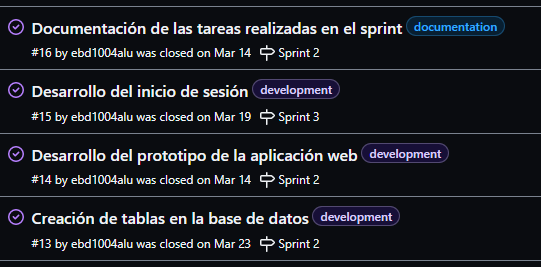
\includegraphics[width=1.0\textwidth]{Sprint2}
    \caption{Issues sprint 2.}
    \label{fig:Sprint2}
\end{figure}
\newpage

En el siguiente gráfico se podría ver el progreso del trabajo durante el sprint, pero debido a un problema que surgió con la herramienta de Zenhub se perdió el progreso de este sprint.
\newpage
\begin{figure}[htb]
    \centering
    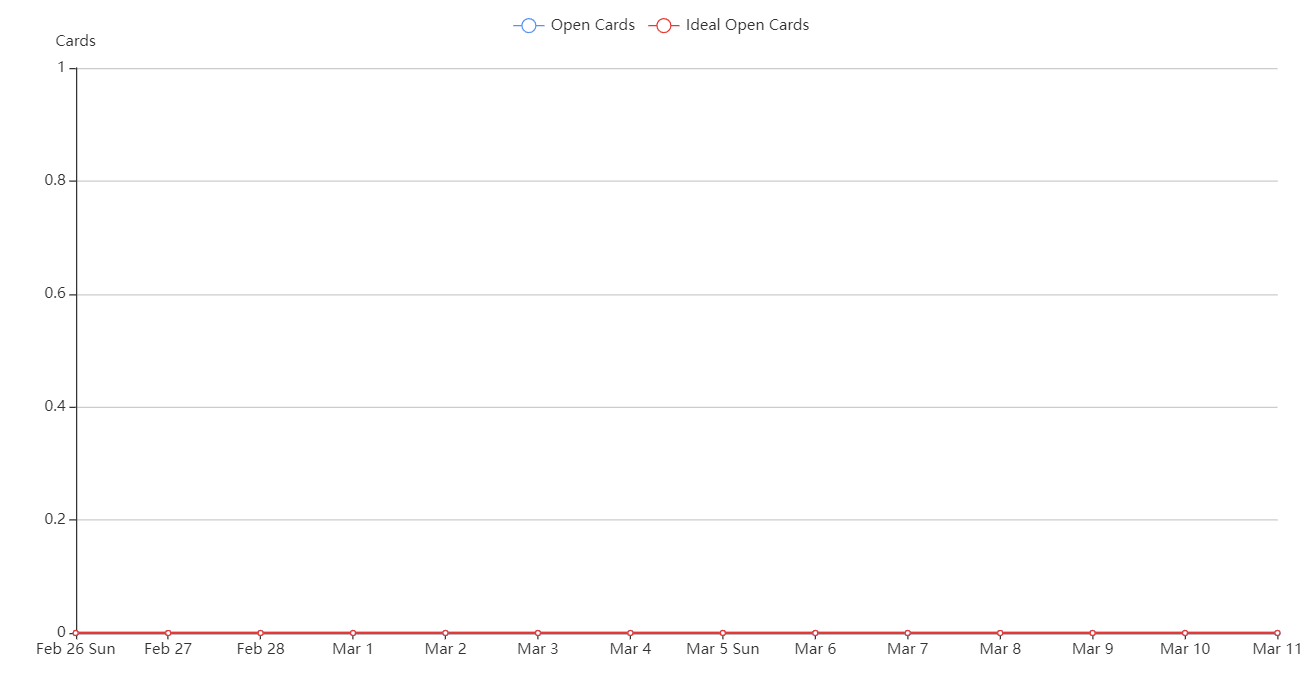
\includegraphics[width=1.1\textwidth]{burndown_2}
    \caption{Burndown del sprint 2.}
    \label{fig:burndown_2}
\end{figure}

\subsection{Sprint 3: 12/03/2023 - 25/03/2023}
La primera semana del sprint 3 fue empleada para seguir con las tareas que no se terminaron en el sprint 2 consistentes en el desarrollo del inicio de sesión y la creación de tablas en la base de datos.

Posteriormente, se realizó el desarrollo del registro y el desarrollo de la vista de inicio.

Por último, se documentaron las tareas realizadas en el sprint.

En este sprint se ha realizado un conjunto de tareas estimadas de 27 story points, y por tanto equivalente a 40 horas y 30 minutos.

\begin{table}[ht!]
    \centering
    \resizebox{15cm}{!} {
    \begin{tabular}{|l|c|c|}
    \hline
    \rowcolor[rgb]{0.99,0.93,0.93}
    \textbf{Tareas}     &\textbf{Tag}     & \textbf{Story points} \\ \hline
    \textbf{Creación de tablas en la base de datos}         &\cellcolor[rgb]{0.99,0.83,0.93}\textcolor{white}{development}      &5 \\ \hline 
    \textbf{Desarrollo de inicio de sesión}         &\cellcolor[rgb]{0.99,0.83,0.93}\textcolor{white}{development}      &8 \\ \hline 
    \textbf{Desarrollo del registro}         &\cellcolor[rgb]{0.99,0.83,0.93}\textcolor{white}{development}      &8 \\ \hline 
    \textbf{Desarrollo de la vista de inicio}         &\cellcolor[rgb]{0.99,0.83,0.93}\textcolor{white}{development}      &5 \\ \hline 
    \textbf{Documentación de las tareas realizadas en el sprint}         &\cellcolor[rgb]{0.0,0.33,0.71}\textcolor{white}{documentation}      &1 \\ \hline 
    \end{tabular}}
    \caption{Tareas completadas del Sprint 3.}
    \label{tab:my_label}
\end{table}

\begin{figure}[htb]
    \centering
    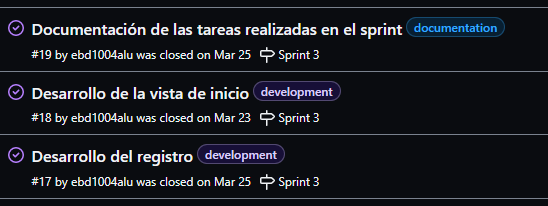
\includegraphics[width=1.0\textwidth]{Sprint3}
    \caption{Issues sprint 3.}
    \label{fig:Sprint3}
\end{figure}

En el siguiente gráfico se podría ver el progreso del trabajo durante el sprint, pero debido a un problema que surgió con la herramienta de Zenhub se perdió el progreso de este sprint.
\begin{figure}[htb]
    \centering
    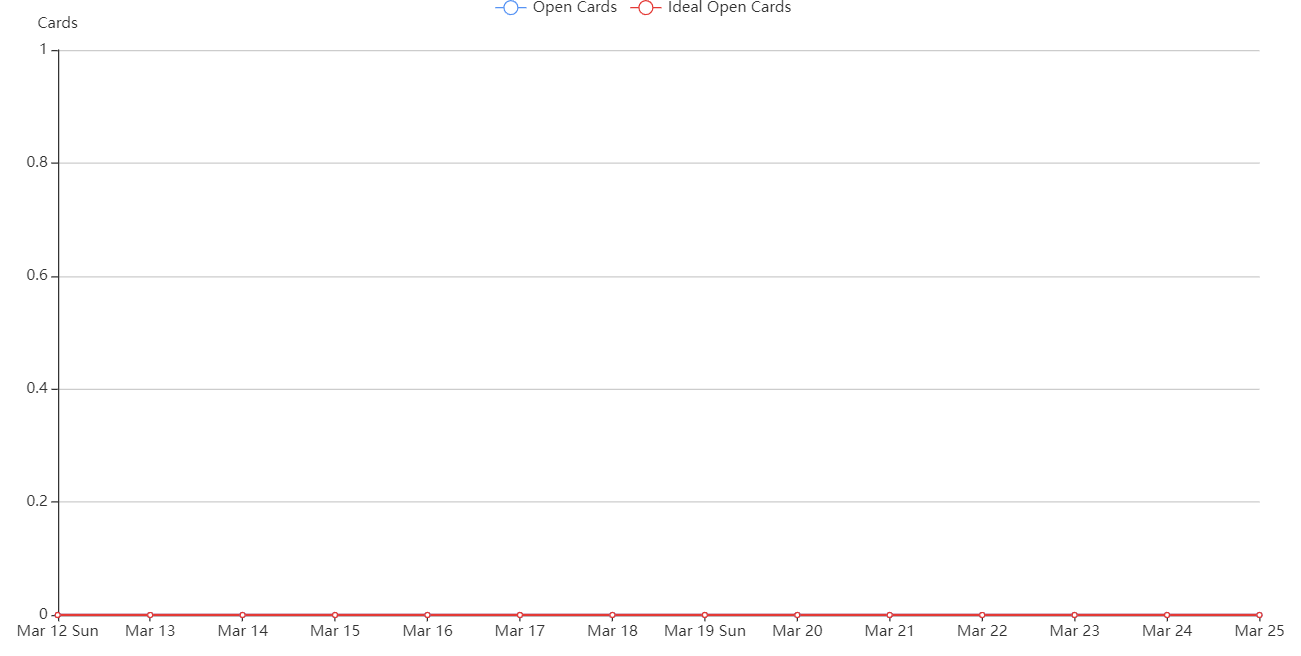
\includegraphics[width=1.1\textwidth]{burndown_3}
    \caption{Burndown del sprint 3.}
    \label{fig:burndown_3}
\end{figure}

\subsection{Sprint 4: 26/03/2023 - 08/04/2023}
La primera semana del sprint 4 fue empleada para realizar la documentación de la memoria empezando por la introducción y después se documentaron los objetivos establecidos del proyecto.

Posteriormente, se realizó el desarrollo del menú de juegos que consistía en la realización de la vista de este menú, y la implementación de una barra de búsqueda y la aplicación de filtros de búsqueda.

Por último, se documentaron las tareas realizadas en el sprint.

En este sprint se ha realizado un conjunto de tareas estimadas de 25 story points, y por tanto equivalente a 26 horas y 30 minutos.

\begin{table}[ht!]
    \centering
    \resizebox{15cm}{!} {
    \begin{tabular}{|l|c|c|}
    \hline
    \rowcolor[rgb]{0.99,0.93,0.93}
    \textbf{Tareas}     &\textbf{Tag}     & \textbf{Story points} \\ \hline
    \textbf{Documentación memoria: Introducción}          &\cellcolor[rgb]{0.0,0.33,0.71}\textcolor{white}{documentation}      &2 \\ \hline 
    \textbf{Documentación memoria: Objetivos del proyecto}          &\cellcolor[rgb]{0.0,0.33,0.71}\textcolor{white}{documentation}      &2 \\ \hline 
    \textbf{Desarrollo del menú de juegos}         &\cellcolor[rgb]{0.99,0.83,0.93}\textcolor{white}{development}      &20 \\ \hline 
    \textbf{Documentación de las tareas realizadas en el sprint}         &\cellcolor[rgb]{0.0,0.33,0.71}\textcolor{white}{documentation}      &1 \\ \hline 
    \end{tabular}}
    \caption{Tareas completadas del Sprint 4.}
    \label{tab:my_label}
\end{table}

\begin{figure}[htb]
    \centering
    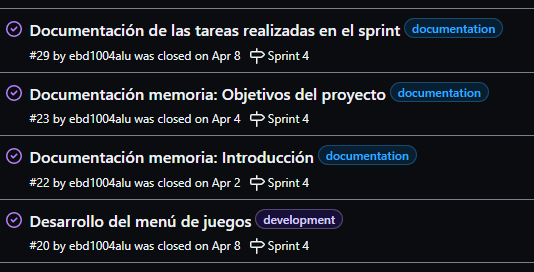
\includegraphics[width=1.0\textwidth]{Sprint4}
    \caption{Issues sprint 4.}
    \label{fig:Sprint4}
\end{figure}
\newpage
En el siguiente gráfico se puede ver el progreso del trabajo durante el sprint.
\begin{figure}[htb]
    \centering
    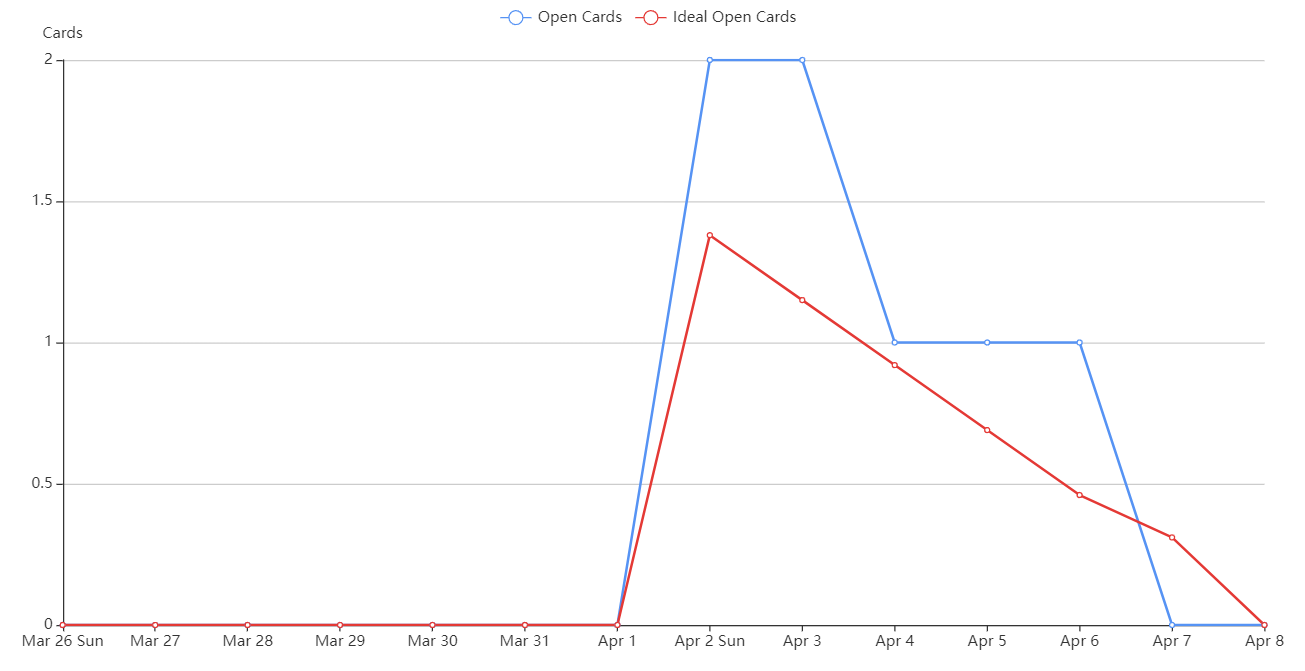
\includegraphics[width=1.0\textwidth]{burndown_4}
    \caption{Burndown del sprint 4.}
    \label{fig:burndown_4}
\end{figure}

\subsection{Sprint 5: 09/04/2023 - 29/04/2023}
La primera semana del sprint 5 se empleó para realizar la documentación de la memoria acerca de las técnicas y herramientas utilizadas para el desarrollo del proyecto, así como los trabajos relacionados con el mismo.

En primer lugar, se trabajó en la paginación del menú de juegos para mejorar la visualización de sus tarjetas. Sin embargo, surgieron inconvenientes durante su implementación, ya que al mostrar los resultados de las búsquedas, ya fuese a través de la barra de búsqueda o mediante la aplicación de filtros, se mostraban tarjetas de juegos que no debían aparecer. Se dedicó el tiempo restante a solucionar este problema, lo que impidió completar las demás tareas previstas para este sprint que tenía una duración de dos semanas.

Por ello, se decidió ampliar una semana más este sprint y así completar las tareas pendientes. Estas tareas incluyeron el desarrollo de la visualización de la infromación de los juegos, la implementación de la funcionalidad que permitiría a los usuarios añadir nuevos juegos, así como permitir la subida de vídeos de YouTube a la aplicación y la implementación de la internacionalización del idioma en la aplicación web.

Por último, se documentaron las tareas realizadas en el sprint.

En este sprint se ha realizado un conjunto de tareas estimadas de 52 story points, y por tanto equivalente a 76 horas y 30 minutos.

\begin{table}[ht!]
    \centering
    \resizebox{15cm}{!} {
    \begin{tabular}{|l|c|c|}
    \hline
    \rowcolor[rgb]{0.99,0.93,0.93}
    \textbf{Tareas}     &\textbf{Tag}     & \textbf{Story points} \\ \hline
    \textbf{Documentación memoria: Técnicas y herramientas}          &\cellcolor[rgb]{0.0,0.33,0.71}\textcolor{white}{documentation}      &3 \\ \hline 
    \textbf{Documentación memoria: Trabajos relacionados}          &\cellcolor[rgb]{0.0,0.33,0.71}\textcolor{white}{documentation}      &3 \\ \hline 
    \textbf{Desarrollo visualización información de juegos}         &\cellcolor[rgb]{0.99,0.83,0.93}\textcolor{white}{development}      &8 \\ \hline
     \textbf{Añadir nuevos juegos}         &\cellcolor[rgb]{0.99,0.83,0.93}\textcolor{white}{development}      &8 \\ \hline 
    \textbf{Añadir vídeos}         &\cellcolor[rgb]{0.99,0.83,0.93}\textcolor{white}{development}      &8 \\ \hline 
    \textbf{Internacionalización}         &\cellcolor[rgb]{0.99,0.83,0.93}\textcolor{white}{development}      &13 \\ \hline 
    \textbf{Paginación menú de juegos}         &\cellcolor[rgb]{0.99,0.83,0.93}\textcolor{white}{development}      &8 \\ \hline 
    \textbf{Documentación de las tareas realizadas en el sprint}         &\cellcolor[rgb]{0.0,0.33,0.71}\textcolor{white}{documentation}      &1 \\ \hline 
    \end{tabular}}
    \caption{Tareas completadas del Sprint 5.}
    \label{tab:my_label}
\end{table}

\begin{figure}[htb]
    \centering
    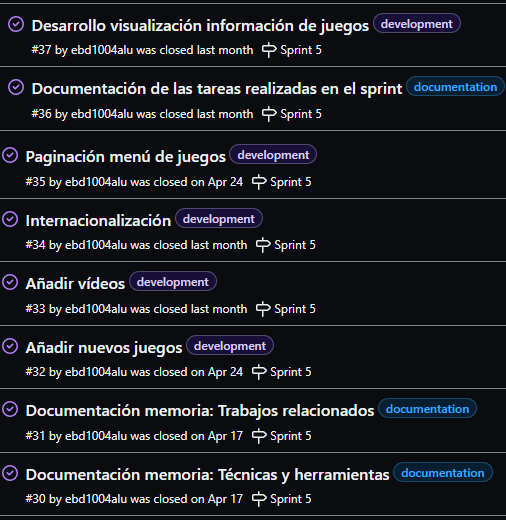
\includegraphics[width=0.7\textwidth]{Sprint5}
    \caption{Issues sprint 5.}
    \label{fig:Sprint5}
\end{figure}

\newpage
En el siguiente gráfico se puede ver el progreso del trabajo durante el sprint.
\begin{figure}[htb]
    \centering
    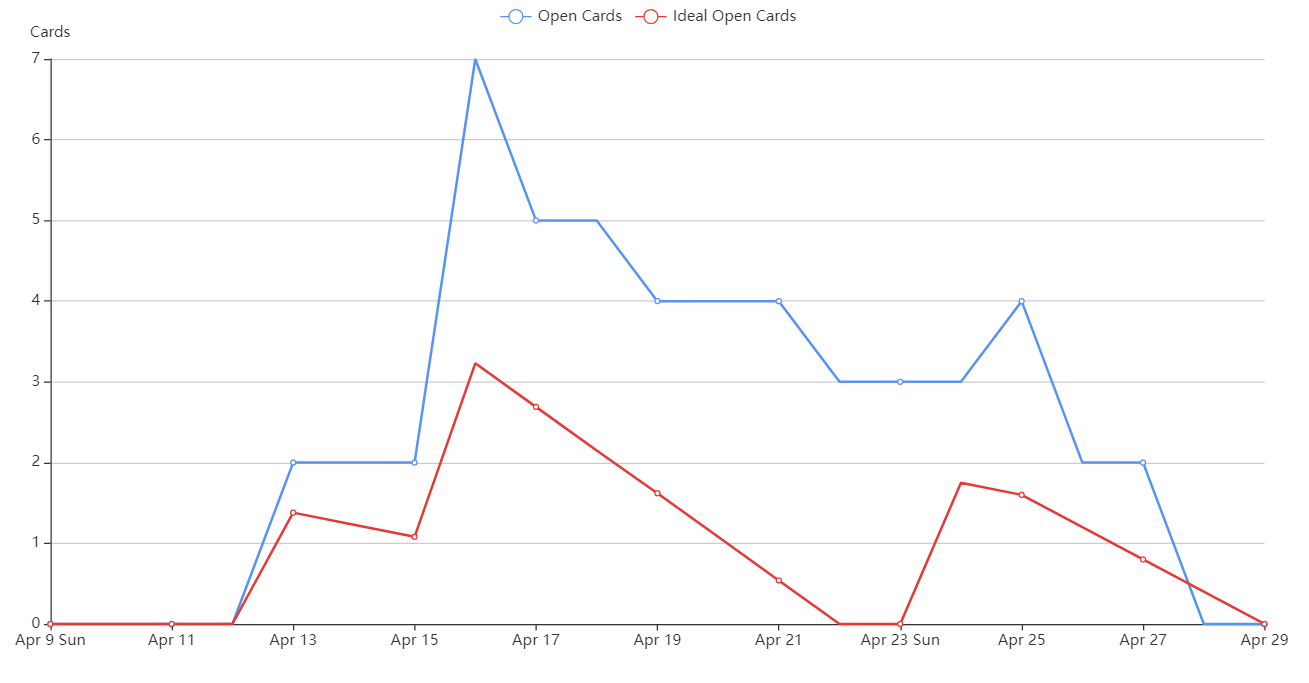
\includegraphics[width=1.0\textwidth]{burndown_5}
    \caption{Burndown del sprint 5.}
    \label{fig:burndown_5}
\end{figure}

\subsection{Sprint 6: 30/04/2023 - 13/05/2023}
La primera semana del sprint 6 se empleó para realizar la implementación que permitiese a los usuarios modificar la información de los juegos de la plataforma y la comprobación de roles. De esta manera, se diferenciaban las funcionalidades según el rol del usuario que se identificaba en la sesión, lo que significaba que solo los usuarios con rol de profesor podían editar y añadir un juego.

Después se implementó la funcionalidad para que un usuario pudiera solicitar el rol de profesor. Para ello, fue necesario crear otra tabla para facilitar el manejo de las solicitudes de los usuarios. De esta manera, los usuarios podían solicitar el rol si aún no lo habían hecho antes, y era el administrador quien tenía la capacidad de administrar las solicitudes pendientes, aceptándolas o rechazándolas, por lo que se implementó el rol de administrador y sus funcionalidades, incluyendo las traducciones de estas para la internacionalización de la aplicación.
Después, se desarrolló la capacidad para que los usuarios pudieran subir y descargar archivos, lo que les permitió incluir instrucciones de los juegos y descargar los juegos en sí mismo.

Posteriormente, se implementó la adaptabilidad de pantalla para que la aplicación pudiera visualizarse correctamente en cualquier dispositivo, junto con el ajuste de los estilos para mejorar la visualización de las interfaces. Además, se implementó que los usuarios pudiesen interactuar con la aplicación a través de valoraciones que incluían añadir una puntuación al juego y una reseña.

Por último, se desarrolló la ventana Acerca de de la aplicación, se documentaron los aspectos relevantes del desarrollo del proyecto y se registraron las tareas realizadas durante el sprint.

En este sprint se ha realizado un conjunto de tareas estimadas de 68 story points, y por tanto equivalente a 99 horas.

\begin{table}[ht!]
    \centering
    \resizebox{15cm}{!} {
    \begin{tabular}{|l|c|c|}
    \hline
    \rowcolor[rgb]{0.99,0.93,0.93}
    \textbf{Tareas}     &\textbf{Tag}     & \textbf{Story points} \\ \hline
    \textbf{Documentación memoria: Aspectos relevantes del desarrollo del proyecto}          &\cellcolor[rgb]{0.0,0.33,0.71}\textcolor{white}{documentation}      &2 \\ \hline 
    \textbf{Modificar juegos}         &\cellcolor[rgb]{0.99,0.83,0.93}\textcolor{white}{development}      &8 \\ \hline
     \textbf{Comprobación de roles}         &\cellcolor[rgb]{0.99,0.83,0.93}\textcolor{white}{development}      &3 \\ \hline 
    \textbf{Implementación de adaptabilidad de pantalla}         &\cellcolor[rgb]{0.99,0.83,0.93}\textcolor{white}{development}      &8 \\ \hline 
    \textbf{Petición para obtener el rol de profesor}         &\cellcolor[rgb]{0.99,0.83,0.93}\textcolor{white}{development}      &13 \\ \hline 
    \textbf{Subir y descargar archivos}         &\cellcolor[rgb]{0.99,0.83,0.93}\textcolor{white}{development}      &8 \\ \hline 
    \textbf{Implementar rol de administrador y sus funcionalidades}         &\cellcolor[rgb]{0.99,0.83,0.93}\textcolor{white}{development}      &8 \\ \hline 
    \textbf{Añadir traducciones de nuevas funcionalidades}         &\cellcolor[rgb]{0.99,0.83,0.93}\textcolor{white}{development}      &3 \\ \hline 
    \textbf{Ajustar estilos para mejorar la visualización}         &\cellcolor[rgb]{0.99,0.83,0.93}\textcolor{white}{development}      &8 \\ \hline 
    \textbf{Añadir valoraciones de usuarios}         &\cellcolor[rgb]{0.99,0.83,0.93}\textcolor{white}{development}      &5 \\ \hline 
    \textbf{Desarrollo acerca de}         &\cellcolor[rgb]{0.99,0.83,0.93}\textcolor{white}{development}      &1 \\ \hline 
    \textbf{Documentación de las tareas realizadas en el sprint}         &\cellcolor[rgb]{0.0,0.33,0.71}\textcolor{white}{documentation}      &1 \\ \hline 
    \end{tabular}}
    \caption{Tareas completadas del Sprint 6.}
    \label{tab:my_label}
\end{table}
\newpage
\begin{figure}[htb]
    \centering
    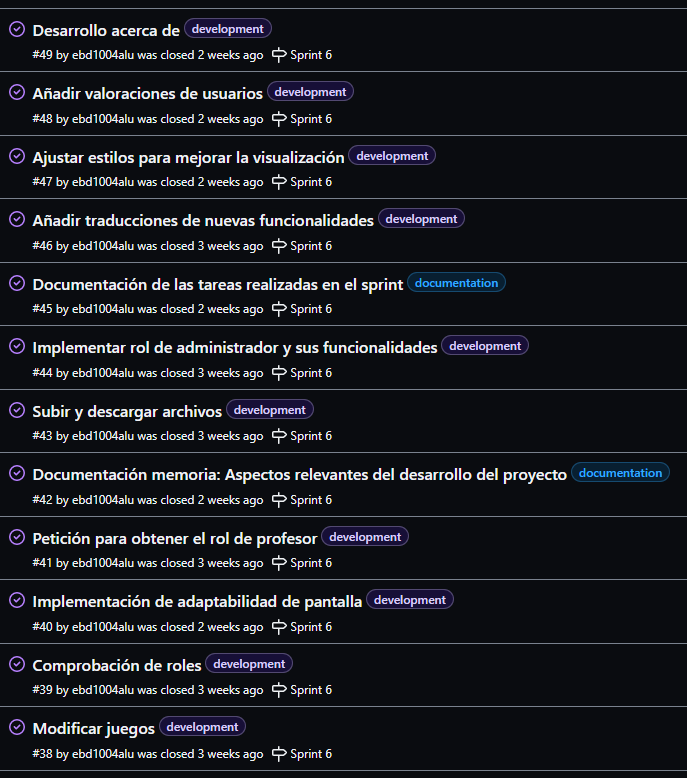
\includegraphics[width=1.0\textwidth]{Sprint6}
    \caption{Issues sprint 6.}
    \label{fig:Sprint6}
\end{figure}
\newpage
En el siguiente gráfico se puede ver el progreso del trabajo durante el sprint.
\begin{figure}[htb]
    \centering
    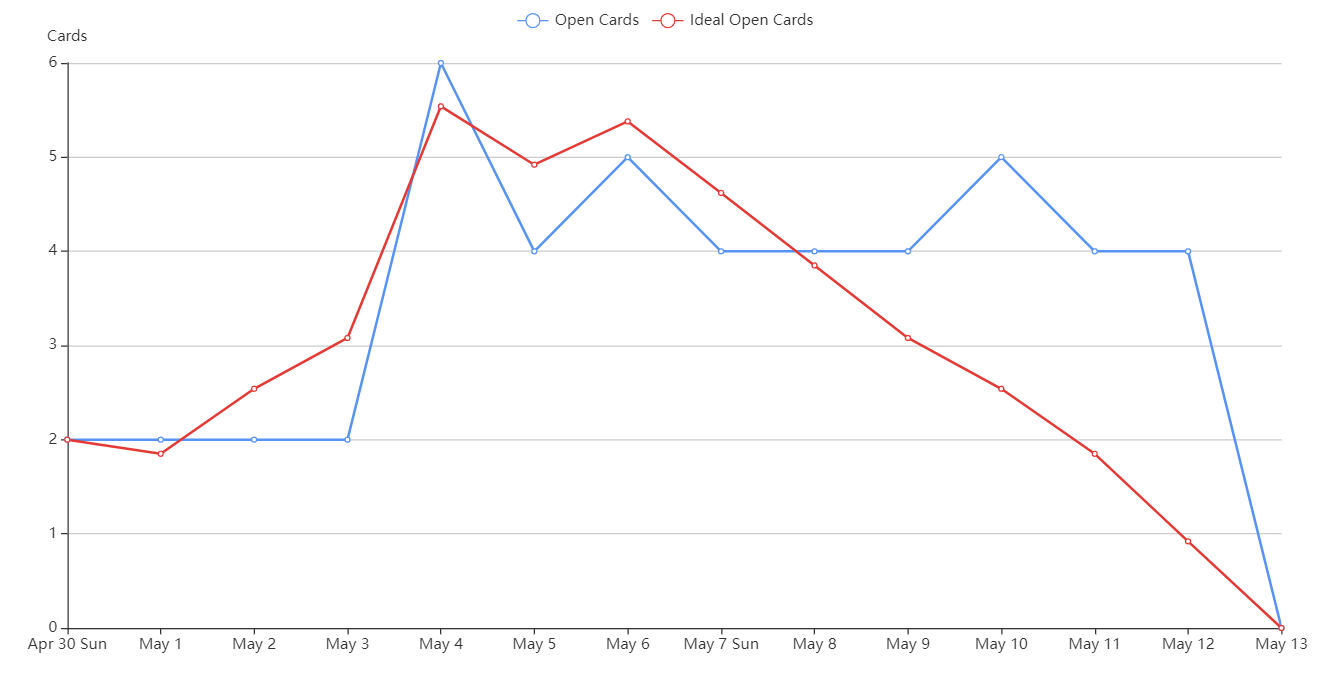
\includegraphics[width=1.0\textwidth]{burndown_6}
    \caption{Burndown del sprint 6.}
    \label{fig:burndown_6}
\end{figure}

\subsection{Sprint 7: 14/05/2023 - 27/05/2023}
La primera semana del sprint 7 se empleó para realizar la documentación de la memoria, incluyendo los conceptos teóricos, las conclusiones y las líneas futuras.

Después, se procedió a añadir las traducciones para las valoraciones restantes y corregir algunos errores (bugs) identificados al probar las funcionalidades de la aplicación. 
El primer error consistía en que los usuarios tenían la posibilidad de descargar archivos, incluso cuando no había ningún archivo disponible para su descarga. Se realizó una corrección en la lógica de la aplicación para solucionar este problema, de manera que ahora la opción de descarga solo se muestra cuando existen archivos disponibles para el usuario.

El segundo error estaba relacionado con la funcionalidad de valoración de los juegos. Los usuarios tenían la posibilidad de valorar un mismo juego repetidamente, lo cual no tenía sentido y podía generar incoherencias en las puntuaciones. Se implementó una corrección en la funcionalidad de valoración para permitir que cada usuario pueda realizar una única valoración por juego, evitando así las valoraciones repetidas.

Posteriormente, se llevaron a cabo los diferentes apartados de los anexos, entre ellos el plan del proyecto, la especificación de requisitos, el diseño, el manual de usuario y el manual del programador.

Por último, se desplegó la aplaicación en Heroku, se realizó el manual de ayuda y se documentaron las tareas realizadas en el sprint.

En este sprint se ha realizado un conjunto de tareas estimadas de 58 story points, y por tanto equivalente a 90 horas.

\begin{table}[ht!]
    \centering
    \resizebox{15cm}{!} {
    \begin{tabular}{|l|c|c|}
    \hline
    \rowcolor[rgb]{0.99,0.93,0.93}
    \textbf{Tareas}     &\textbf{Tag}     & \textbf{Story points} \\ \hline
    \textbf{Documentación memoria: Conceptos teóricos }          &\cellcolor[rgb]{0.0,0.33,0.71}\textcolor{white}{documentation}      &5 \\ \hline 
    \textbf{Documentación memoria: Conclusiones y líneas futuras}         &\cellcolor[rgb]{0.0,0.33,0.71}\textcolor{white}{documentation}      &2 \\ \hline
     \textbf{Añadir traducciones para valoraciones}         &\cellcolor[rgb]{0.99,0.83,0.93}\textcolor{white}{development}      &1 \\ \hline 
    \textbf{Documentación anexos: Requisitos}         &\cellcolor[rgb]{0.0,0.33,0.71}\textcolor{white}{documentation}      &8 \\ \hline 
    \textbf{Permite descargar archivo y no hay archivo subido}         &\cellcolor[rgb]{0.8, 0.36, 0.36}\textcolor{white}{bug}      &1 \\ \hline 
    \textbf{Permite valorar juegos repetidamente}         &\cellcolor[rgb]{0.8, 0.36, 0.36}\textcolor{white}{bug}      &1 \\ \hline 
    \textbf{Documentación anexos: Diseño}         &\cellcolor[rgb]{0.0,0.33,0.71}\textcolor{white}{documentation}      &13 \\ \hline 
    \textbf{Documentación anexos: Manual usuario}         &\cellcolor[rgb]{0.0,0.33,0.71}\textcolor{white}{documentation}      &5 \\ \hline 
    \textbf{Documentación anexos: Manual programador}         &\cellcolor[rgb]{0.0,0.33,0.71}\textcolor{white}{documentation}      &5 \\ \hline 
    \textbf{Despliegue de la aplicación en Heroku}         &\cellcolor[rgb]{0.99,0.83,0.93}\textcolor{white}{development}      &8 \\ \hline 
    \textbf{Manual de ayuda}         &\cellcolor[rgb]{0.0,0.33,0.71}\textcolor{white}{documentation}      &5 \\ \hline 
    \textbf{Documentación anexos: Plan proyecto}         &\cellcolor[rgb]{0.0,0.33,0.71}\textcolor{white}{documentation}      &8 \\ \hline 
    \textbf{Documentación de las tareas realizadas en el sprint}         &\cellcolor[rgb]{0.0,0.33,0.71}\textcolor{white}{documentation}      &1 \\ \hline 
    \end{tabular}}
    \caption{Tareas completadas del Sprint 7.}
    \label{tab:my_label}
\end{table}
\newpage
\begin{figure}[htb]
    \centering
    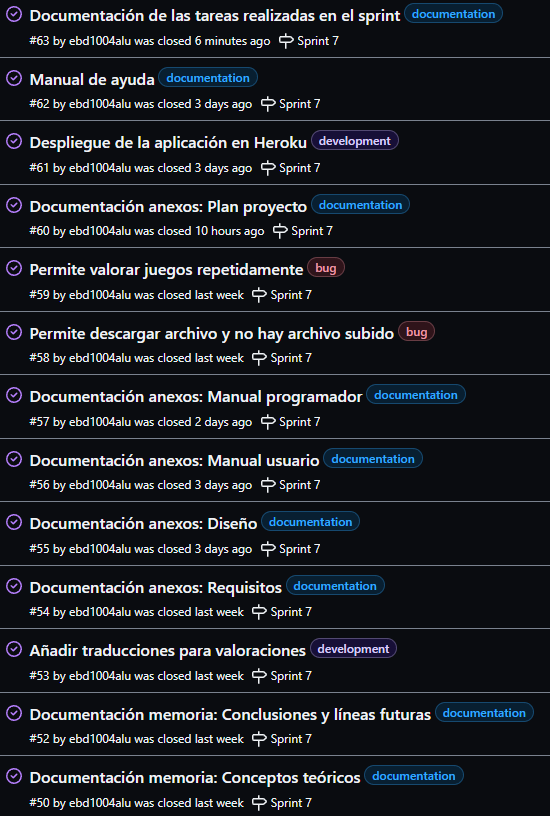
\includegraphics[width=0.7\textwidth]{Sprint7}
    \caption{Issues sprint 7.}
    \label{fig:Sprint7}
\end{figure}
\newpage
En el siguiente gráfico se puede ver el progreso del trabajo durante el sprint.
\begin{figure}[htb]
    \centering
    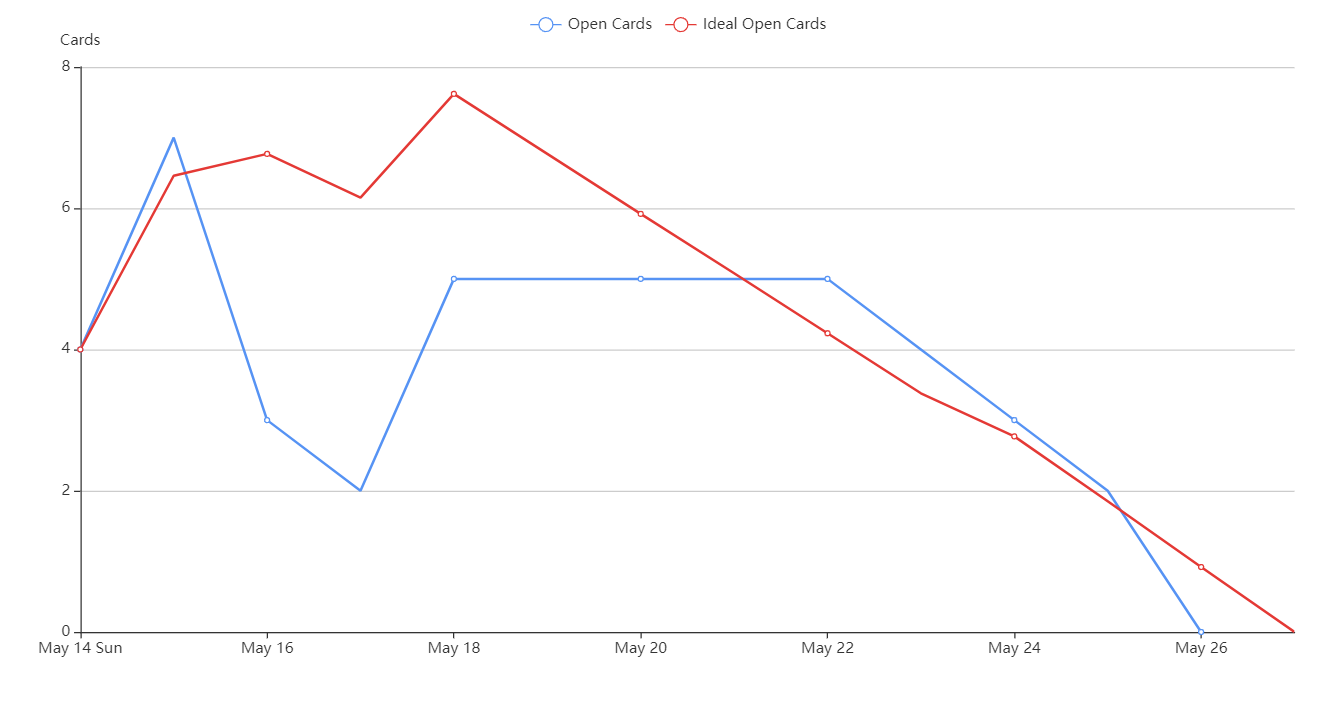
\includegraphics[width=1.0\textwidth]{burndown_7}
    \caption{Burndown del sprint 7.}
    \label{fig:burndown_7}
\end{figure}

\subsection{Sprint 8: 28/05/2023 - 03/06/2023}

\section{Estudio de viabilidad}
El estudio de la viabilidad del proyecto es fundamental para determinar su factibilidad y asegurar su éxito.
Este incluye un estudio de la viabilidad económica y de la viabilidad legal bajo un supuesto desarrollo en el mercado real.

\subsection{Viabilidad económica}
La viabilidad económica implica el análisis de los costes y beneficios asociados al desarrollo del proyecto.

\subsubsection{Costes}
Los costes asociados al desarrollo de un proyecto se pueden clasificar generalmente en tres categorías principales: costes de personal, costes de hardware y costes de software.

\begin{itemize}
    \item \textbf{Costes de personal:} los costes de personal se calculan teniendo en cuenta que el alumno ha realizado unas 500 horas totales de trabajo repartidas aproximadamente en 4 meses, por lo que ha empleado aproximadamente 31 horas semanales, dependiendo de la carga de tareas de cada semana.

Se estima que el sueldo del alumno va a ser 17€/hora, por lo que el salario mensual bruto es 2108€ al mes:

$$ 31\frac{horas}{semana}\times17\frac{\text{\euro}}{hora}\times4\frac{semanas}{mes}=2108\text{\euro}\hspace{0.5em}al\hspace{0.5em}mes  $$

Además, se deben pagar una serie de impuestos a la seguridad social que se pueden consultar en la página oficial de la Seguridad Social: \url{https://www.seg-social.es/wps/portal/wss/internet/Trabajadores/CotizacionRecaudacionTrabajadores/36537}

\begin{enumerate}
    \item Contingencias comunes: costes asociados con circunstancias de incapacidad temporal o permanente debido a enfermedad común, accidentes no laborales y lesiones.
    \imagen{tipos-cotizacion}{Tipos de cotización.}
    \item Desempleo: costes por el desempleo de un trabajador.
    \imagen{desempleo}{Desempleo.}
    \item Fondo de Garantía Salarial (FOGASA): se encarga de garantizar el pago de salarios e indemnizaciones a los trabajadores cuando los empleadores no pueden hacerlo por insolvencia o concurso de acreedores.
    \imagen{FOGASA}{FOGASA.}
    \item Formación profesional: costes por las necesidades de formación del trabajador.
    \imagen{formacion-profesional}{Formación profesional.}
\end{enumerate}

Los costes que tendría la empresa al contratar al alumno serían los siguientes:

    \begin{table}[h]
    \centering
    \begin{tabular}{p{8cm}rrr}
        \hline
        \textbf{Concepto económico} & \textbf{Coste} \\
        \hline
        Salario mensual neto & 2108€/mes  \\
        Contingencias comunes (23,6\%) & 497,49€ \\
        Desempleo (5,5\%)  & {115,94€/mes}\\
        FOGASA (0,2\%) & {4,22€/mes}\\
        Formación profesional (0,6\%) & {12,65€/mes}\\\hline
        Salario mensual bruto  & {2.770,33€/mes}\\
        \hline
        Coste 4 meses  & {\textbf{11.081,32€/4 meses}}\\
        \hline
    \end{tabular}
    \caption{Costes del personal.}
    \label{tab:costes-software}
\end{table}
\newpage
La dedicación de los tutores del proyecto no se ha considerado como un coste a tener en cuenta al tratarse de la tutorización del trabajo de fin de grado.

\item \textbf{Costes de hardware:} el hardware que se ha utilizado para el desarrollo del proyecto ha sido un ordenador portátil Lenovo Ideapad, un monitor AOC y como periféricos necesarios, un teclado y un ratón.

La vida útil estimada del hardware empleada es de 5 años, por lo que cada año se amortiza el 20 \% del valor del hardware. La duración del proyecto ha sido de 4 meses, y por tanto las amortizaciones calculadas son:

\begin{table}[h]
    \centering
    \begin{tabular}{p{4cm}rrr}
        \hline
        \textbf{Hardware} & \textbf{Coste} & \textbf{Amortización} & \textbf{Valor contable final} \\
        \hline
        Portátil Lenovo & 520€ & 34,68€ & 485,32€ \\
        Monitor AOC & 150€ & 10€ & 140€ \\
        Periféricos & 30€ & 2€ & 28€ \\
        \hline
        \textbf{Total} & 700€ & 46,68€ & 653,32€ \\
        \hline
    \end{tabular}
    \caption{Costes de hardware}
    \label{tab:costes-hardware}
\end{table}

La amortización se ha calculado de la siguiente forma:
\begin{itemize}
    \item \textbf{Portátil Lenovo} 
    
El coste anual de amortización es: 
    \begin{center}
        $$ 20\% \times 520 \text{\euro} = 104 \text{\euro} $$
    \end{center}
    
El coste anual de amortización se divide en partes iguales entre los 12 meses del año, lo que da como resultado una amortización mensual de: 

    \begin{center}
       {\Large\(\frac{104\text{€}}{\text{12 meses}}\)} = 8,67 {\Large\(\frac{\text{€}}{\text{mes}}\)}
    \end{center}

Por lo tanto, para los 4 meses del proyecto, la amortización total para el portátil Lenovo sería: 

    \begin{center}
        $$ 8,67\frac{\text{\euro}}{mes}\times4\hspace{0.5em}meses=34,68\text{\euro}  $$
    \end{center}

    \item \textbf{Monitor AOC} 

    El coste anual de amortización es: 

    \begin{center}
        $$ 20\% \times 150 \text{\euro} = 30 \text{\euro} $$
    \end{center}
    
    El coste anual de amortización se divide en partes iguales entre los 12 meses del año, lo que da como resultado una amortización mensual de: 

    \begin{center}
        $$ \frac{30 \text{\euro}}{12 \hspace{0.5em}meses}=2,50\frac{\text{\euro}}{mes}  $$
    \end{center}

    Por lo tanto, para los 5 meses del proyecto, la amortización total para los periféricos sería: 

    \begin{center}
        $$ 2,50\frac{\text{\euro}}{mes}\times4\hspace{0.5em}meses=10\text{\euro}  $$
    \end{center}

    \item \textbf{Periféricos} 

    El coste anual de amortización es:  

    \begin{center}
        $$ 20\% \times 30 \text{\euro} = 6 \text{\euro} $$
    \end{center}
    
    El coste anual de amortización se divide en partes iguales entre los 12 meses del año, lo que da como resultado una amortización mensual de: 

    \begin{center}
        $$ \frac{6 \text{\euro}}{12 \hspace{0.5em}meses}=0,50\frac{\text{\euro}}{mes}  $$
    \end{center}

    Por lo tanto, para los 5 meses del proyecto, la amortización total para el monitor AOC sería: 

    \begin{center}
        $$ 0,50\frac{\text{\euro}}{mes}\times4\hspace{0.5em}meses=2\text{\euro}  $$
    \end{center}
\end{itemize}

El valor contable al final del proyecto se ha calculado de la siguiente forma:
\begin{itemize}
    \item \textbf{Portátil Lenovo} 
    
    La amortización total para los 4 meses del proyecto es de 34,68€. Por lo tanto, el valor contable del portátil al final del proyecto sería: 

    \begin{center}
        520€ - 34,68€ = 485,32€
    \end{center}

    \item \textbf{Monitor AOC} 

    La amortización total para los 4 meses del proyecto es de 10€. Por lo tanto, el valor contable del monitor al final del proyecto sería: 

    \begin{center}
        150€ - 10€ = 140€
    \end{center}

    \item \textbf{Periféricos}
    
    La amortización total para los 4 meses del proyecto es de 2€. Por lo tanto, el valor contable de los periféricos al final del proyecto sería: 

    \begin{center}
        30€ - 2€ = 28€
    \end{center}
\end{itemize}

\item \textbf{Costes de software:} para el desarrollo del proyecto se utilizó Heroku tanto para el despliegue de la aplicación web como para la base de datos. Al disponer de la cuenta de estudiante de GitHub se obtuvieron unos créditos para usar en la plataforma de Heroku de forma gratuita por lo que no se tuvieron costes.

La mayoría de herramientas que se han empleado son de código abierto y gratuitas, por lo que no se consideran coste de software.

\item \textbf{Costes totales:} los costes totales se calculan sumando el total de los costes de hardware, software y personal.
    \begin{table}[h]
    \centering
    \begin{tabular}{p{6cm}rrr}
        \hline
        \textbf{Concepto económico} & \textbf{Coste} \\
        \hline
        Costes del personal & 11.081,32€ \\
        Costes del hardware & 700€ \\
        Costes del software & 0€ \\
        \hline
        Total  & {\textbf{11.781,32€}}\\
        \hline
    \end{tabular}
    \caption{Costes totales.}
    \label{tab:costes-totales}
\end{table}
\end{itemize}

\subsection{Beneficios}
La aplicación web se publica de manera gratuita ya que al tratarse de un proyecto de carácter educativo no se busca obtener beneficios económicos con su lanzamiento.

\subsection{Viabilidad legal}
La viabilidad legal trata de identificar las distintas licencias que requieren las herramientas empleadas para  cumplir con los requisitos legales durante el desarrollo del proyecto.

Las licencias y versiones de las herramientas usadas son las siguientes:
\begin{table}[ht!]
    \centering
    \resizebox{13cm}{!} {
    \begin{tabular}{|l|l|l|}
    \hline
         \textbf{Herramienta/Librería}     &  \textbf{Versión}   &\textbf{Licencia} \\ \hline
         {Flask}       & {2.2.3 }  &{BSD-3-Clause} \\ \hline
         {Flask-Login}       & {0.6.2}  &{MIT} \\ \hline
         {GitHub}       & {3.1.2}    &{GNU} \\ \hline 
         {Heroku}       & {-}    &{ISC} \\ \hline 
         {PostgreSQL}       & {6.18 }    &{PostgreSQL License} \\ \hline 
         {Bootstrap}       & {12.16.1}    &{MIT} \\ \hline 
         {Werkzeug}       & {2.3.3}    &{BSD-3-Clause} \\ \hline 
         {psycopg2-binary}       & {2.9.5 }    &{LGPL} \\ \hline 
         {Dotenv}       & {0.21.0 }    &{BSD-2-Clause Simplified} \\ \hline 
         {Unidecode}       & {1.3.6}    &{GNU} \\ \hline 
         {gunicorn}       & {20.1.0}    &{MIT} \\ \hline 
    \end{tabular}}
    \caption{Tabla de licencias}
    \label{tab:licencias}
\end{table}

A continuación se detallan las características y la función de las licencias de las herramientas utilizadas:

\begin{enumerate}
    \item\textbf{GNU} \textit{(General Public License)} \cite{gnu} licencia de software libre que permite a los usuarios usar, modificar y distribuir el software. Sin embargo, el software derivado debe disponer de los mismos términos que el original.
    
    \item \textbf{BSD} \textit{(Berkeley Source Distribution)} \cite{bsd} licencia de software de código abierto que permite a los usuarios el uso, modificación y distribución del software sin restricciones adicionales. A diferencia con la licencia GPL acepta el uso del código fuente en software no libre.
    
    
    \item \textbf{BSD-2-Clause Simplified} \textit{(Berkeley Source Distribution 2)} \cite{bsd-2} licencia de código abierto que permite a los usuarios el uso, modificación y distribución del software. Las distribuciones deben disponer del aviso de derechos del autor anterior y la lista de condiciones de responsabilidad en las distribuciones del software.
    
    \item \textbf{BSD-3-Clause} \textit{(Berkeley Source Distribution 3)} \cite{bsd-3}
licencia de código abierto que permite a los usuarios el uso, la distribución y modificación del software. Las distribuciones deben disponer del aviso de derechos del autor anterior y la lista de condiciones de responsabilidad en la documentación y/o en otros materiales.

    \item \textbf{ISC} \textit{(Internet Systems Consortium)} licencia de código abierto que permite a los usuarios usar, modificar y distribuir el software sin restricciones, aunque en las distribuciones se requiere el aviso de los derechos del autor original.
     
    \item \textbf{PostgreSQL License} \cite{postgresql-license} licencia de código abierto que permite a los usuarios usar, modificar y distribuir el software de PostgreSQL.
    
    \item \textbf{MIT} \textit{(Massachusetts Institute of Technology)}  \cite{mit} licencia que concede el permiso, a cualquier usuario que obtenga una copia del software y de los archivos de documentación asociados, los derechos de usar, copiar, publicar, modificar, fusionar, distribuir y/o vender copias del software.
    
    \item \textbf{LGPL} \textit{(Lesser General Public License)} \cite{lgpl} licencia de código abierto que permite a los usuarios el uso, modificación y distribución de bibliotecas LGPL sin necesidad de que todo el proyecto se licencie bajo sus términos. Únicamente los elementos derivados del proyecto requerirán seguir la licencia.
    
\end{enumerate}